% Fig 2.8 (formerly numbered 2.14) -- cdf of a mixed random variable
%             (manuscript mathstatch2.tex lines 961-978, Example 2.13)
% F(x) = 0 for x<0, 1-0.8e^{-x} for x>=0; jump of 0.2 at x=0, asymptote 1.
% Drawing scale: y=3 corresponds to probability 1 (same scale as Figs A01, A03)
%
% Type size, and the one deviation from CH2_FIGURE_SPECS.md 3.3.1:
%   The 3.3.1 spec sizes the type for a display width of 350px, the plain
%   topic-figure--wide case.  The figure has since been moved inside the
%   Example 2.13 box, where the figure element measures 309px on a 390px
%   phone, and at 309px the \small annotation fell to 11.98px, under the 12px
%   floor of spec 1.3.  The class option is therefore 11pt rather than the
%   default 10pt, which makes \normalsize 10.95pt and \small 10pt.  Native
%   size 231.829 x 138.729 pt (was 231.289 x 136.542; the drawing is 8.04cm
%   wide, inside the 9.0cm cap), so at 309px
%       \normalsize 10.95pt -> 14.54px
%       \small      10pt    -> 13.28px
%   Geometry is untouched: every coordinate, the endpoints, the two y ticks,
%   the jump arrow and the curve are exactly as 3.3.1 specifies.
%   The X of F_X stays at scriptscript size (6pt, 7.97px at 309px).  It is a
%   component of the symbol, not a label, and every other cdf figure on the
%   site sets it the same way; lifting it is a site-wide decision, not one to
%   take in a single file.
\documentclass[tikz,border=2pt,11pt]{standalone}
\usepackage{amsmath}
\usepackage{amssymb}
\usepackage{xcolor}
\usetikzlibrary{arrows.meta}
\newcommand{\sssig}{\scriptscriptstyle}

\definecolor{journalink}{HTML}{1F1C18}
\definecolor{journalmuted}{HTML}{8A7F72}
\definecolor{journalaccent}{HTML}{9C2D2D}

\begin{document}
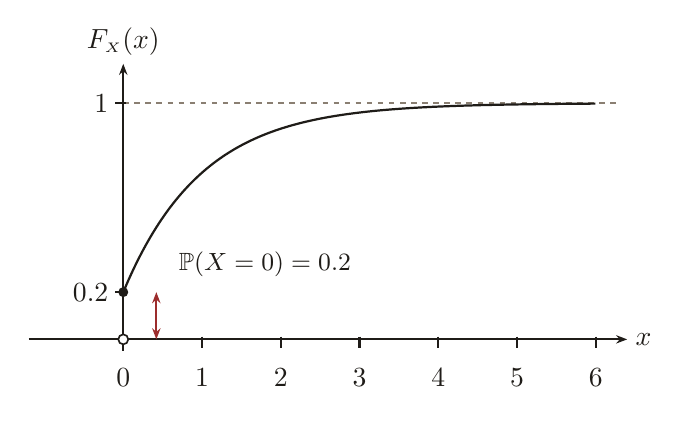
\begin{tikzpicture}[
  x=1cm,
  y=1cm,
  every node/.style={font=\normalsize, journalink},
  axis/.style={journalink, line width=0.8pt, -{Stealth[length=4pt]}},
  tick/.style={journalink, line width=0.8pt},
  curve/.style={journalink, line width=0.8pt},
  guide/.style={journalmuted, line width=0.5pt, dash pattern=on 2pt off 2pt},
  jump/.style={journalaccent, line width=0.8pt,
               {Stealth[length=4pt]}-{Stealth[length=4pt]}},
  solidpt/.style={circle, fill=journalink, inner sep=0pt, minimum size=3.6pt},
  openpt/.style={circle, draw=journalink, line width=0.6pt, fill=white,
                 inner sep=0pt, minimum size=3.6pt}
]
  % ---- axes (x axis starts at -1.2 so the flat piece for x<0 is visible) ----
  \draw[axis] (-1.2,0) -- (6.4,0);
  \draw[axis] (0,0) -- (0,3.5);

  % ---- horizontal asymptote (probability 1) ----
  \draw[guide] (0,3) -- (6.3,3);

  % ---- x ticks (the tick at x=0 is lengthened to clear the open endpoint) ----
  \draw[tick] (0,0.035) -- (0,-0.150);
  \foreach \x in {1,2,3,4,5,6}
    \draw[tick] (\x,0.035) -- (\x,-0.106);
  \foreach \x in {0,1,2,3,4,5,6}
    \node[anchor=north] at (\x,-0.25) {$\x$};

  % ---- y ticks: 0.6 corresponds to 0.2, and 3 to 1 ----
  \draw[tick] (0.035,0.6) -- (-0.106,0.6) node[anchor=east, inner sep=2pt] {$0.2$};
  \draw[tick] (0.035,3)   -- (-0.106,3)   node[anchor=east, inner sep=2pt] {$1$};

  % ---- cdf: flat piece for x<0 ----
  \draw[curve] (-1.2,0) -- (0,0);

  % ---- cdf: continuous rise 3(1-0.8e^{-x}) for x>=0 ----
  \draw[curve] plot[domain=0:6, samples=200, smooth]
    (\x, {3*(1-0.8*exp(-\x))});

  % ---- jump-height annotation ----
  \draw[jump] (0.42,0) -- (0.42,0.6);
  \node[anchor=west, inner sep=0pt] at (0.70,0.95)
    {\small $\mathbb{P}(X=0)=0.2$};

  % ---- endpoints (drawn last, on top of the segments) ----
  \node[openpt]  at (0,0)   {};
  \node[solidpt] at (0,0.6) {};

  % ---- axis labels ----
  \node[anchor=west, inner sep=2.8pt] at (6.4,0) {$x$};
  \node[anchor=south, inner sep=0pt] at (0,3.6) {$F_{\sssig X}(x)$};
\end{tikzpicture}
\end{document}
